\documentclass{standalone}

\usepackage{tikz}
\usepackage{circuitikz}

\tikzset{block/.style = {draw, fill=white, very thick, rectangle, minimum height=1cm, minimum width=2cm},
         lblock/.style={draw,fill=white,very thick, rectangle, minimum height=3cm, minimum width=1cm},
         sum/.style= {draw, fill=white, very thick, circle, node distance=0.5cm}}

         
\begin{document}
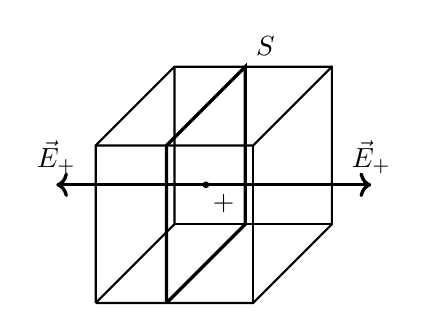
\begin{tikzpicture}[scale=2]
    \draw[-, thick](0,0)--(1,0)--(1.5,0.5)--(1.5,1.5)--(0.5,1.5)--(0,1)--(0,0);
    \draw[-, thick](0,0)--(0.5,0.5)--(0.5,1.5);
    \draw[-, thick](0.5,0.5)--(1.5,0.5);
    \draw[-, thick](0,1)--(1,1)--(1.5,1.5);
    \draw[-, thick](1,1)--(1,0);
    \draw[-,very thick](0.45,0)--(0.95,0.5)node[above left]{$+$}--(0.95,1.5)node[above right]{$S$}--(0.45,1)--(0.45,0);

    \filldraw[black](0.7,0.75)circle(0.5pt);
    \draw[->,very thick](0.7,0.75)--(1.75,0.75)node[above]{$\vec{E}_+$};
    \draw[->,very thick](0.7,0.75)--(-0.25,0.75)node[above]{$\vec{E}_+$};
\end{tikzpicture}
\end{document}